\documentclass[tikz,border=8pt]{standalone}
\usepackage{amsmath}
\usetikzlibrary{arrows.meta,calc}

\definecolor{latticeblue}{RGB}{52,101,164}
\definecolor{pointred}{RGB}{198,40,40}
\definecolor{guidegray}{RGB}{105,105,105}

\begin{document}
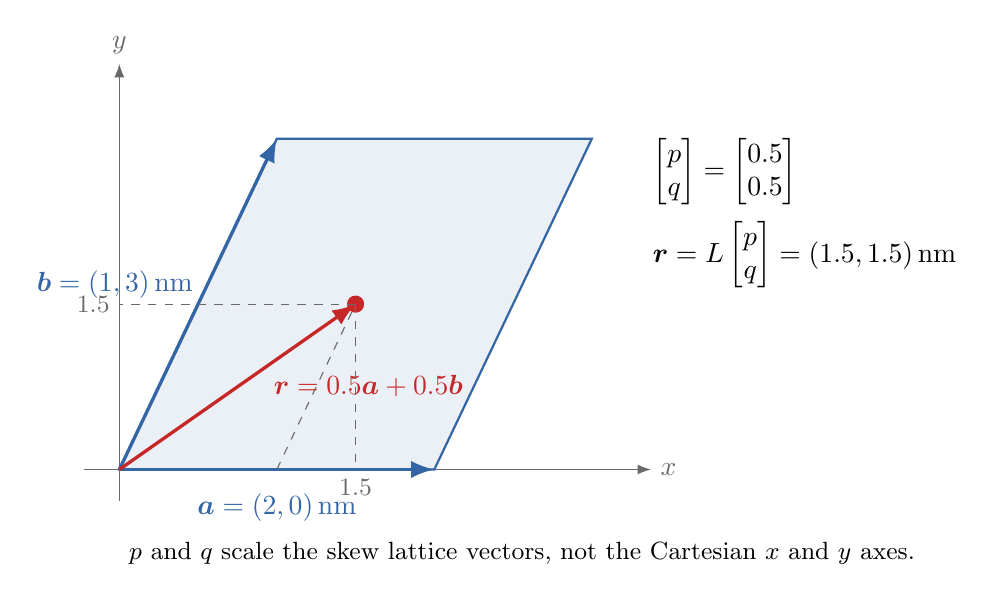
\begin{tikzpicture}[
  >=Latex,
  axis/.style={->, thin, guidegray},
  cell/.style={latticeblue, thick},
  lattice vector/.style={->, very thick, latticeblue},
  position vector/.style={->, very thick, pointred},
  guide/.style={dashed, thin, guidegray},
  label/.style={font=\small}
]

\coordinate (O) at (0,0);
\coordinate (A) at (4,0);
\coordinate (B) at (2,4.2);
\coordinate (AB) at ($(A)+(B)$);
\coordinate (R) at ($(O)!0.5!(AB)$);
\coordinate (HA) at ($(O)!0.5!(A)$);
\coordinate (HB) at ($(O)!0.5!(B)$);

% Cartesian axes and one skew unit cell.
\draw[axis] (-0.45,0) -- (6.75,0) node[right] {$x$};
\draw[axis] (0,-0.4) -- (0,5.15) node[above] {$y$};
\fill[latticeblue!10] (O) -- (A) -- (AB) -- (B) -- cycle;
\draw[cell] (O) -- (A) -- (AB) -- (B) -- cycle;

% Lattice vectors are the columns of L.
\draw[lattice vector] (O) -- (A)
  node[midway, below=5pt] {$\boldsymbol a=(2,0)\,\mathrm{nm}$};
\draw[lattice vector] (O) -- (B)
  node[midway, above left=-2pt] {$\boldsymbol b=(1,3)\,\mathrm{nm}$};

% Half of each lattice vector constructs r.
\draw[guide] (HA) -- (R);
\draw[guide] (HB) -- (R);
\draw[position vector] (O) -- (R)
  node[pos=0.62, below right=-1pt] {$\boldsymbol r=0.5\boldsymbol a+0.5\boldsymbol b$};
\fill[pointred] (R) circle (3.1pt);

\draw[guide] (R) -- ($(R |- O)$)
  node[below, label] {$1.5$};
\draw[guide] (R) -- ($(O |- R)$)
  node[left, label] {$1.5$};

\node[align=left, anchor=west] at (6.65,3.25)
  {$\begin{bmatrix}p\\q\end{bmatrix}
    =\begin{bmatrix}0.5\\0.5\end{bmatrix}$\\[5pt]
   $\boldsymbol r=L\begin{bmatrix}p\\q\end{bmatrix}
    =(1.5,1.5)\,\mathrm{nm}$};

\node[label, anchor=north west] at (0,-0.8)
  {$p$ and $q$ scale the skew lattice vectors, not the Cartesian $x$ and $y$ axes.};

\end{tikzpicture}
\end{document}
